\documentclass{beamer}
\mode<presentation>
\usepackage[english]{babel}
\usepackage{graphicx}
\usepackage{libertine}

\title{Version control with Git}
\author{Etienne Dysli Metref}
\date{January 2016}

\AtBeginSection[]
{
  \begin{frame}<beamer>{Outline}
    \tableofcontents[currentsection,hideothersubsections]
  \end{frame}
}

\begin{document}
\begin{frame}
  \titlepage
\end{frame}

\begin{frame}{Outline}
  \tableofcontents[hideallsubsections]
\end{frame}

\section{Version control}
\begin{frame}{What is version control?}
  \begin{block}{Record changes made to files over time}
    \begin{itemize}
    \item ``Go back in time'', revert files to previous version
    \item Compare versions, find differences
    \end{itemize}
  \end{block}
  \begin{block}{Collaboration tool}
    \begin{itemize}
    \item Easily share files and changes
    \item Parallel lines of development
    \end{itemize}
  \end{block}
\end{frame}

\begin{frame}{Centralized vs. distributed systems}
  \begin{columns}[t]
    \begin{column}{5.5cm}
      \begin{block}{Centralized}
        \begin{itemize}
        \item Examples: CVS, Subversion, Perforce
        \item Clients check out the latest version from a server
        \item Needs a connection to the server for all operations
        \item One place to go to
        \end{itemize}
      \end{block}
    \end{column}
    \begin{column}{5.5cm}
      \begin{block}{Distributed}
        \begin{itemize}
        \item Examples: Git, Mercurial, Bazaar
        \item Clients download a complete copy of the repository
        \item Works without a network connection
        \item Requires some organization: where is the reference?
        \end{itemize}
      \end{block}
    \end{column}
  \end{columns}
\end{frame}

\section{Git concepts}

\begin{frame}{Distributed}
  Everyone has a complete copy of the repository
  \begin{center}
    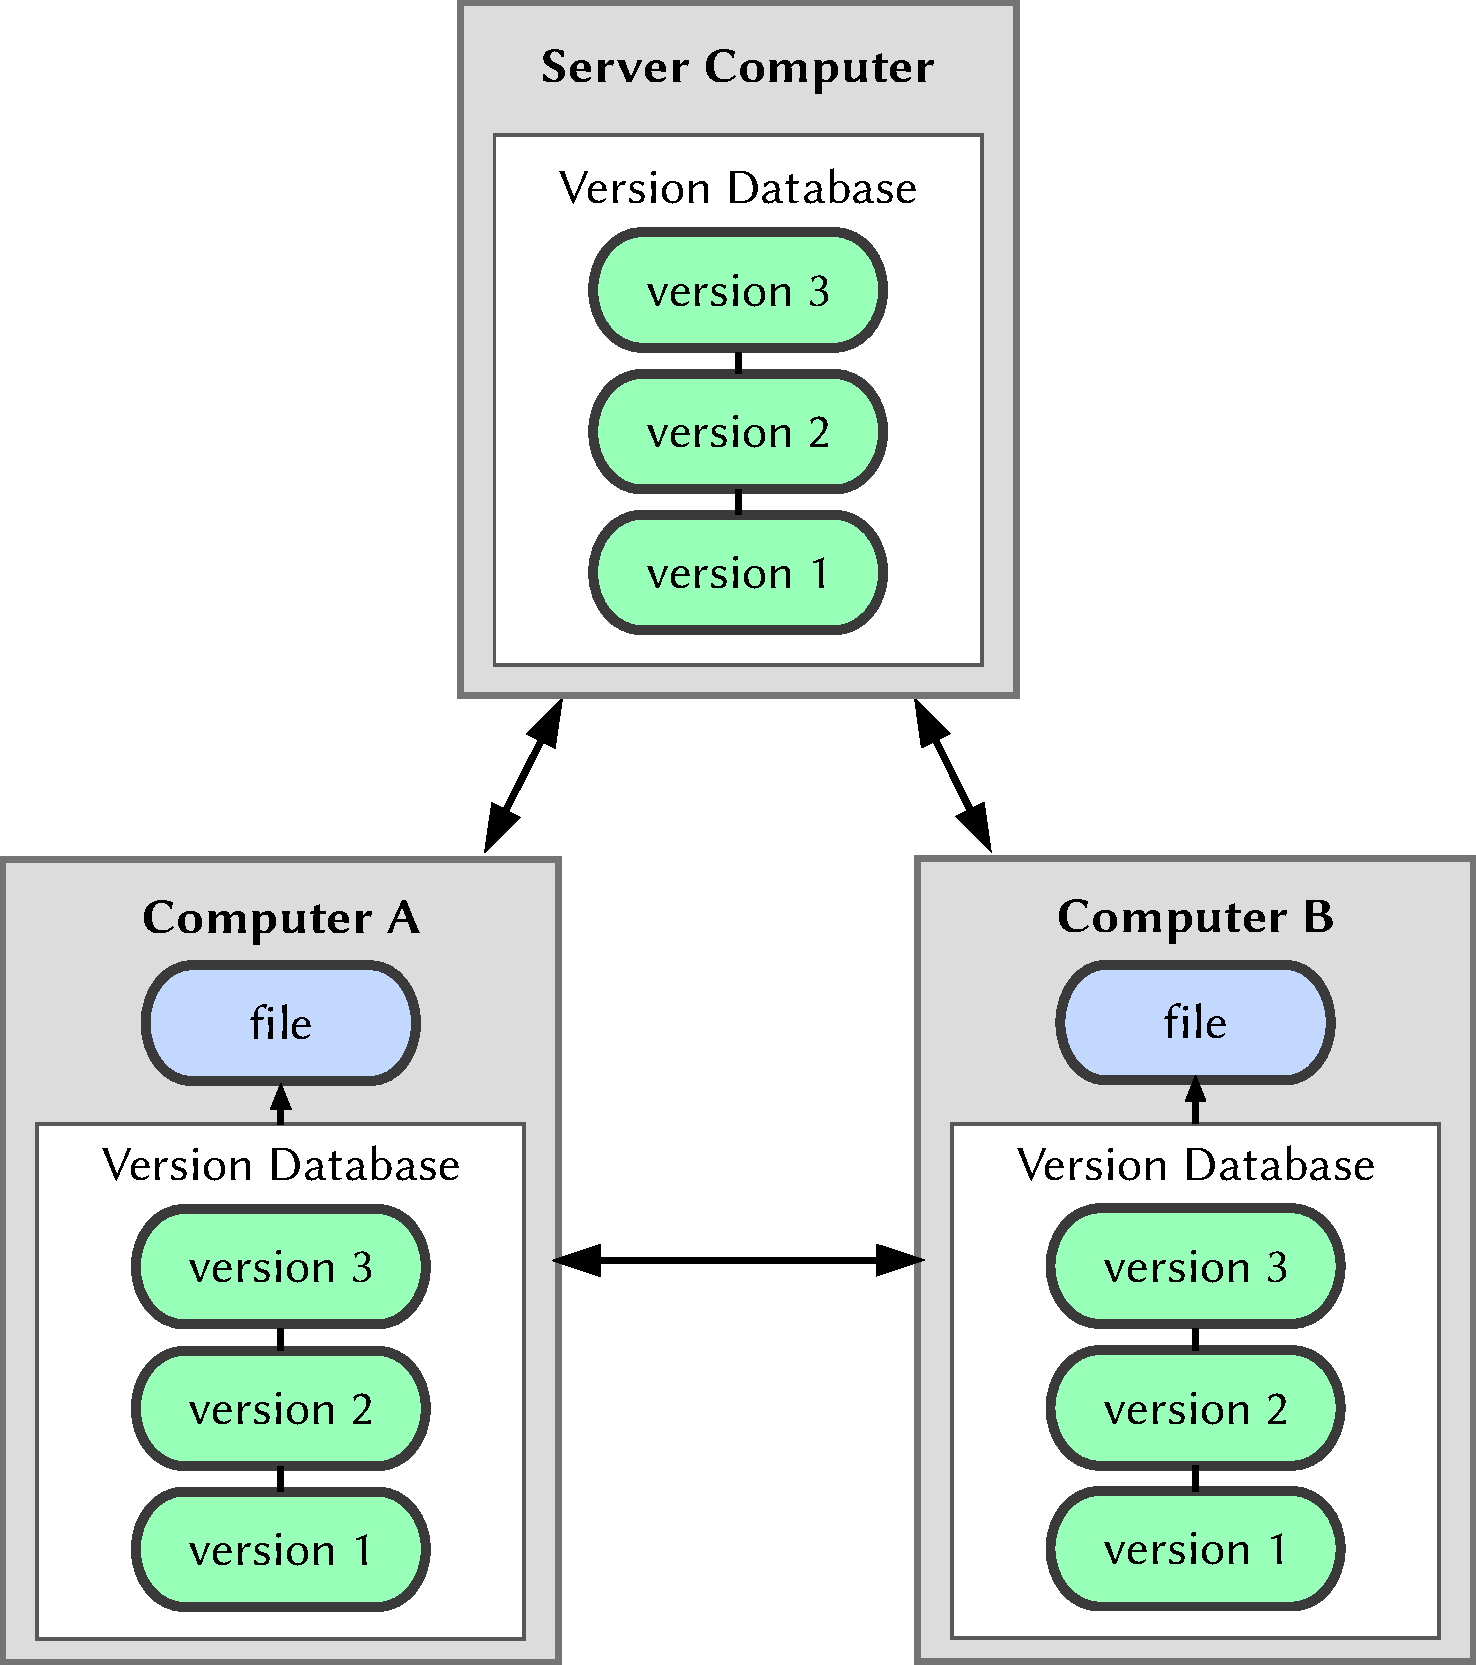
\includegraphics[height=7cm]{images/fig0103.pdf}
  \end{center}
\end{frame}

\begin{frame}{Inside a Git-managed project}
The .git directory is the \emph{repository}, everything else is the \emph{working directory}.
  \begin{center}
    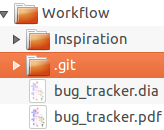
\includegraphics{images/directory_structure.png}
  \end{center}
\end{frame}

\begin{frame}{Commits}
  \begin{center}
    \only<+>{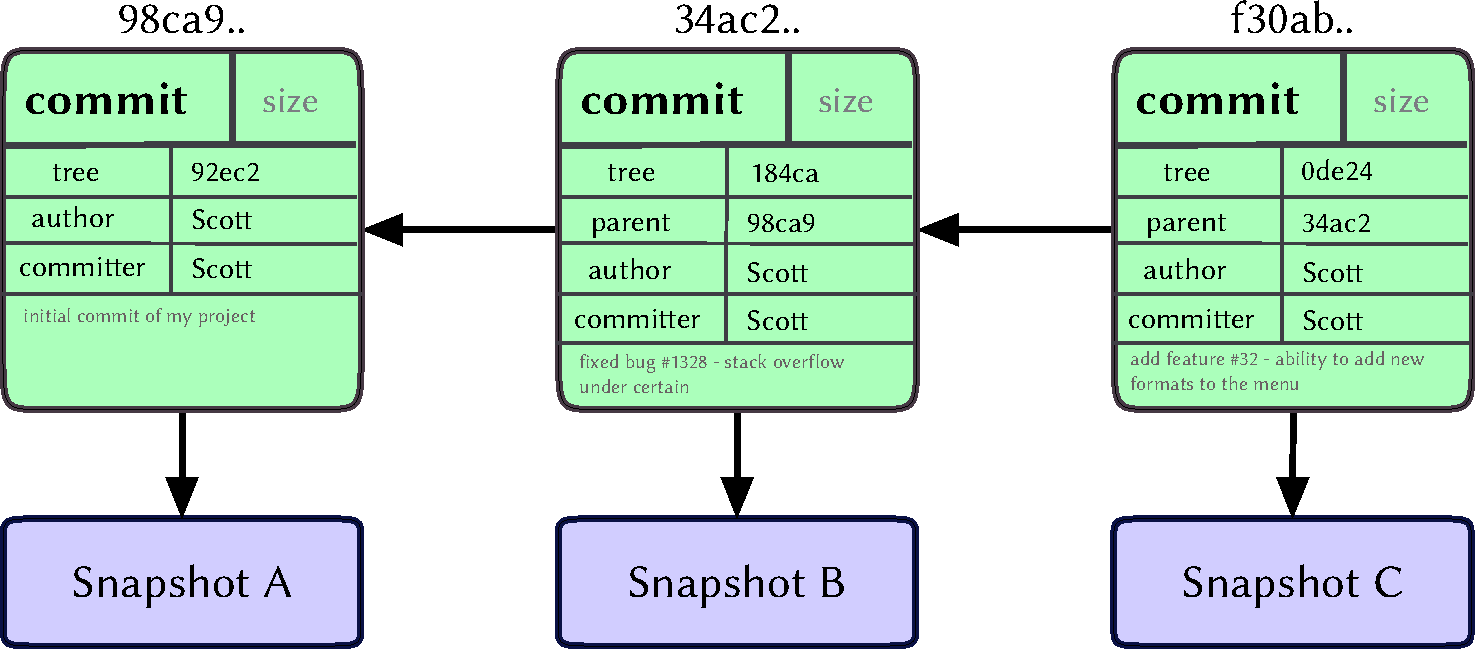
\includegraphics[height=4cm]{images/fig0302.pdf}}
  \end{center}
  \begin{itemize}
  \item Git stores whole files in the repository, not differences
  \item A \emph{commit} is a snapshot of tracked files at given time
  \item Each commit is identified by its hash (SHA-1), no sequential revision numbers
  \item Commits contain pointers to their parent commit(s)
  \end{itemize}
\end{frame}

\begin{frame}{The staging area and file states}
  \begin{center}
    \only<+>{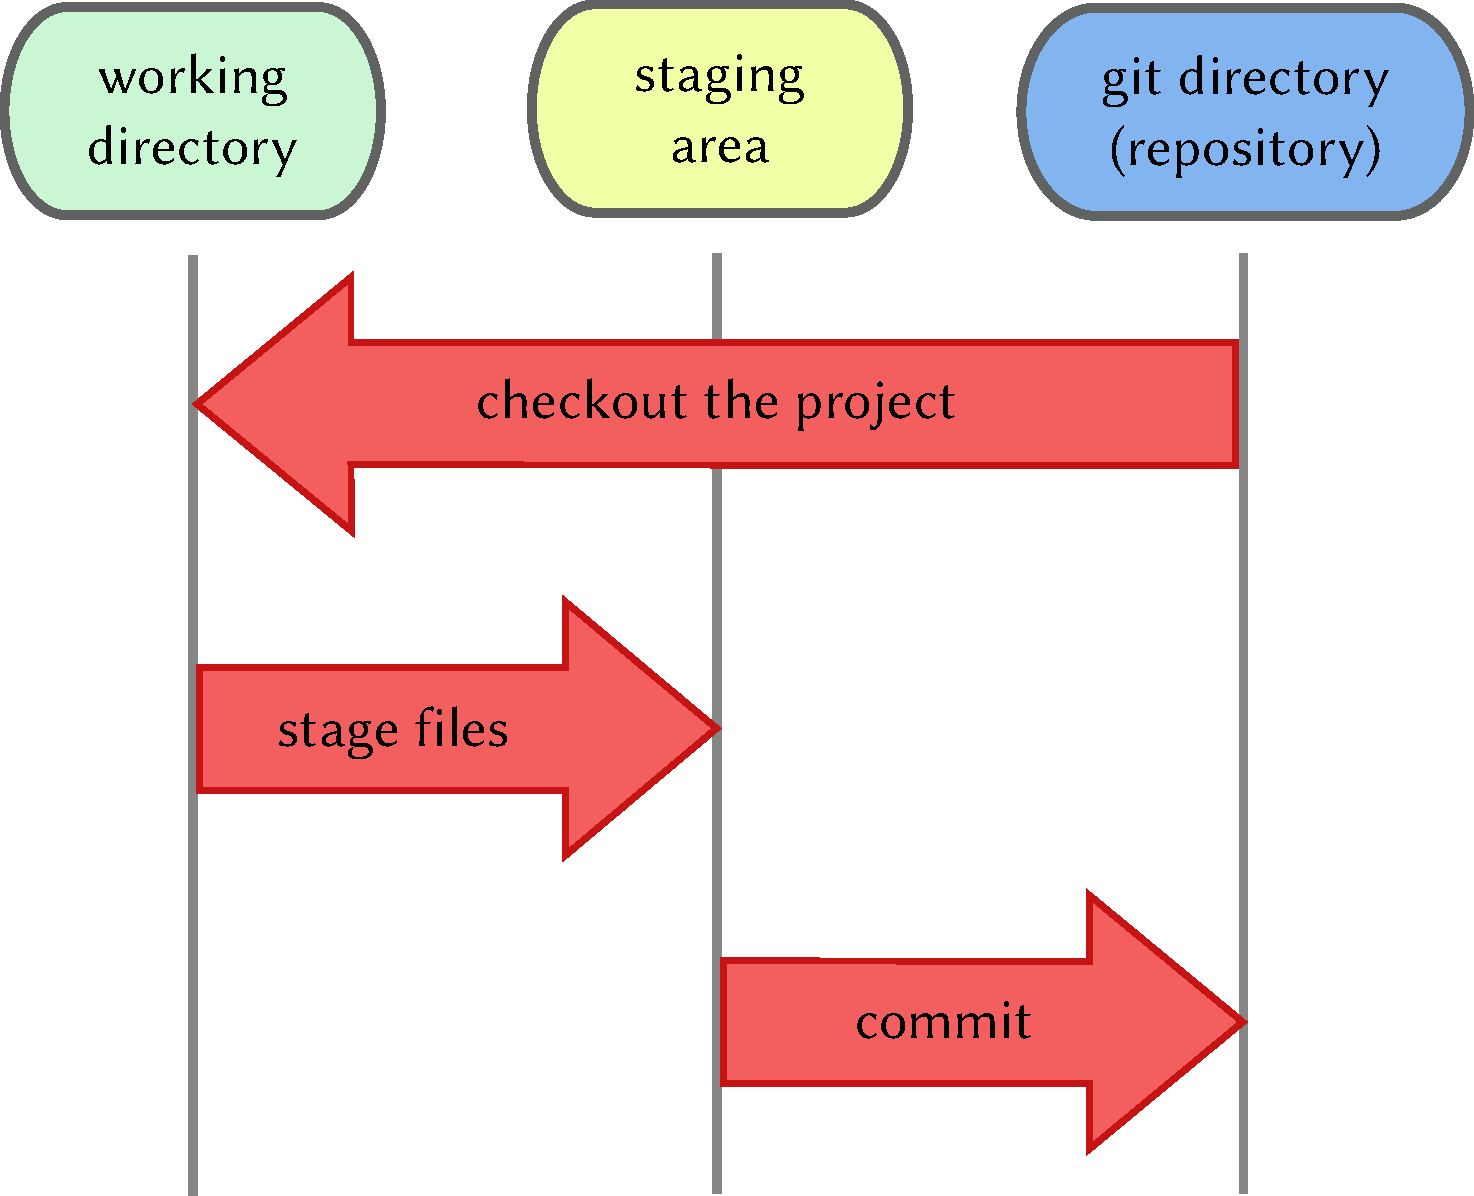
\includegraphics[height=7cm]{images/fig0106.pdf}}
    \only<+>{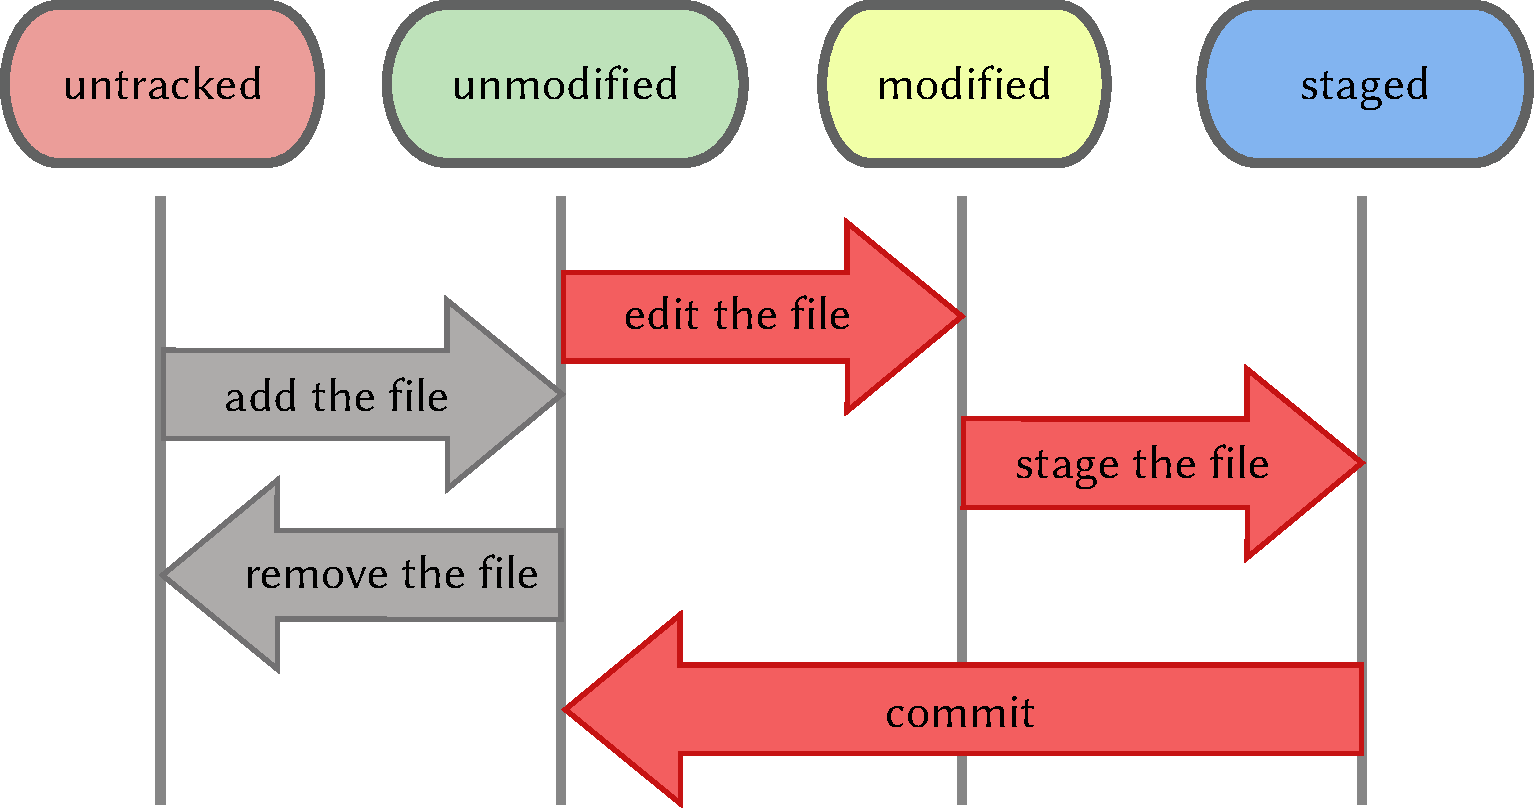
\includegraphics[width=10.8cm]{images/fig0201.pdf}}
  \end{center}
\end{frame}

\begin{frame}{Branches}
  \begin{center}
    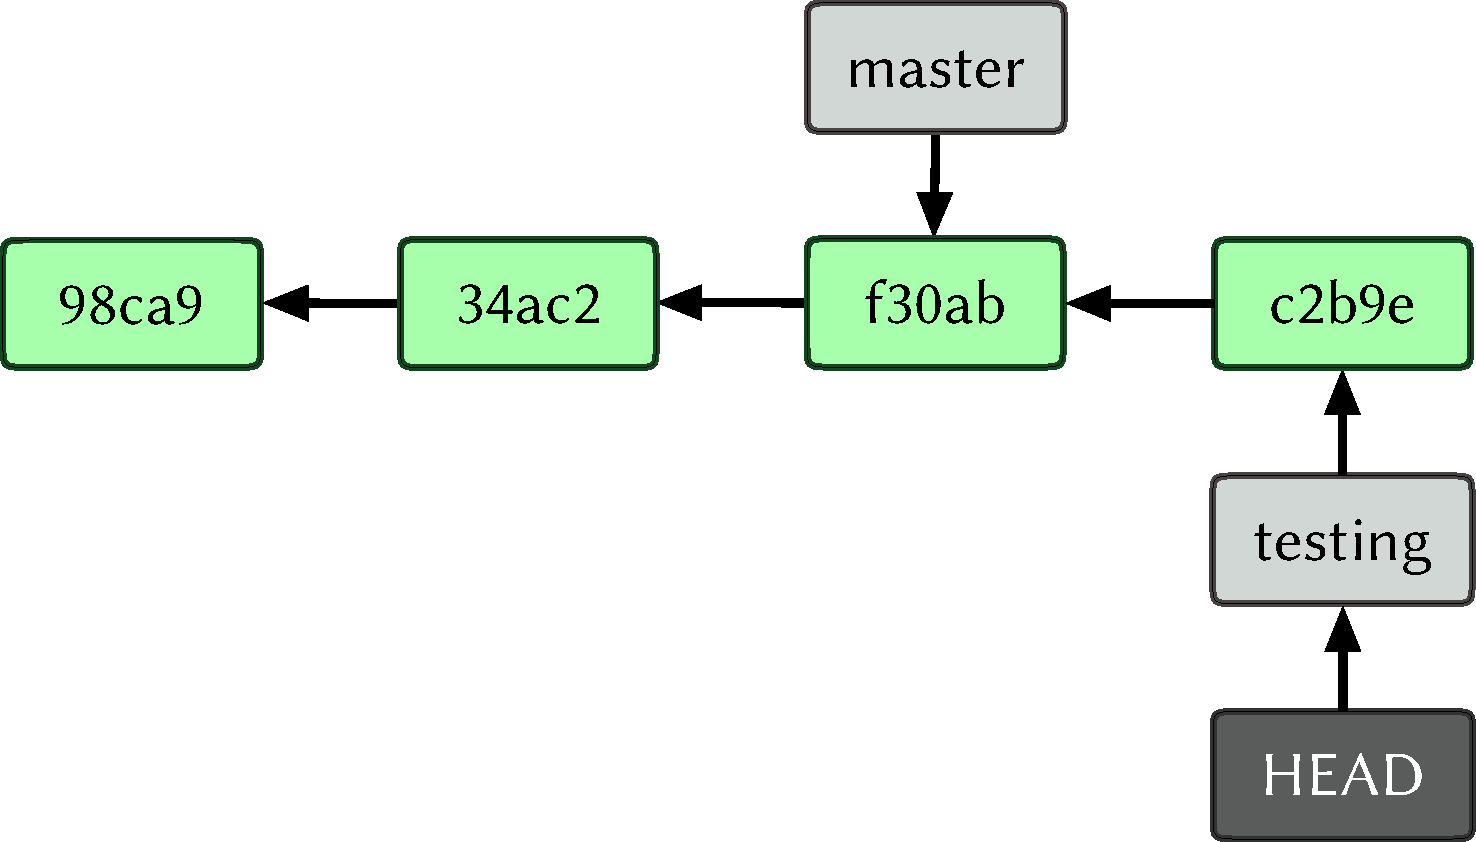
\includegraphics[height=4cm]{images/fig0307.pdf}
  \end{center}
  \begin{itemize}
  \item[Branch] Pointer to a commit\\Very fast to create, delete or modify
  \item[master] Default branch name
  \item[HEAD] Points to the current branch
  \end{itemize}
\end{frame}

\begin{frame}{Merging}
  \begin{itemize}
  \item Fast and easy: ``just'' moving branch pointers around
  \item Two types of merge: \emph{fast-forward} and \emph{three-way}\\Git automatically picks the appropriate way
  \item Using only fast-forward merges makes the history nicely linear and easy to follow
  \item When conflicts happen, they still need to be manually resolved
  \item \emph{Rebasing} helps keeping the history linear
  \end{itemize}
\end{frame}

\begin{frame}{Merging: fast-forward}
  \begin{center}
    \only<+>{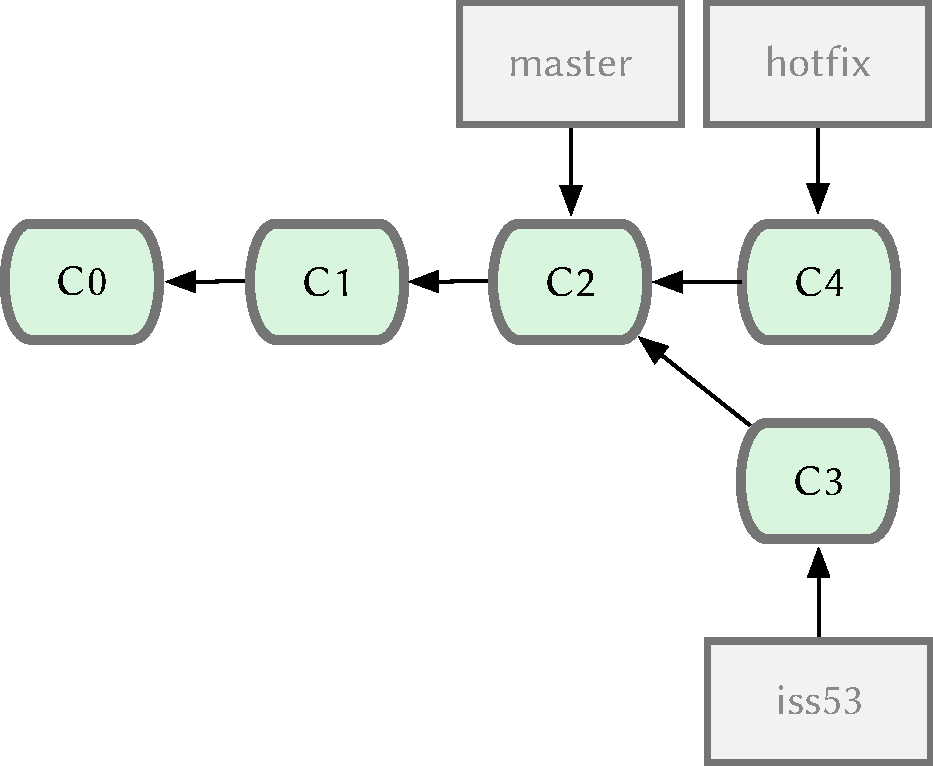
\includegraphics[scale=0.4]{images/fig0313.pdf}}
    \only<+>{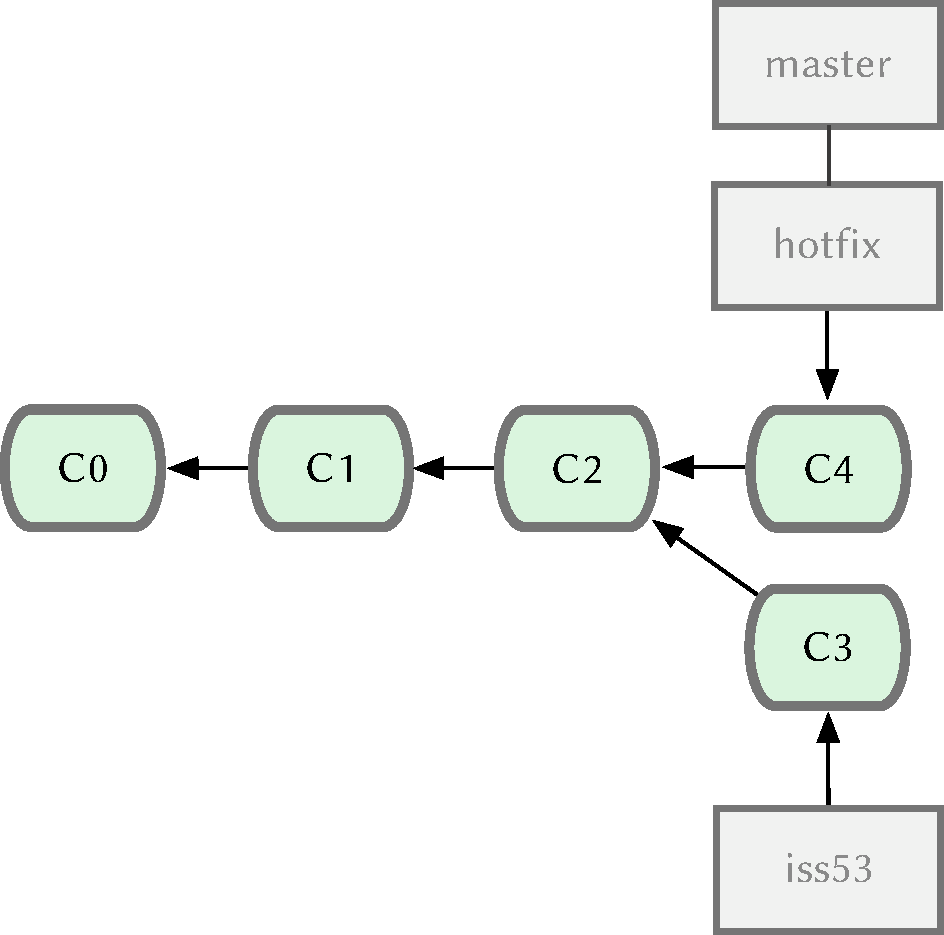
\includegraphics[scale=0.4]{images/fig0314.pdf}}
  \end{center}
  \begin{itemize}
  \item Merge hotfix into master = move the branch pointer forward
  \item There cannot be conflicts in this case
  \end{itemize}
\end{frame}

\begin{frame}{Merging: three-way}
  \begin{center}
    \only<+>{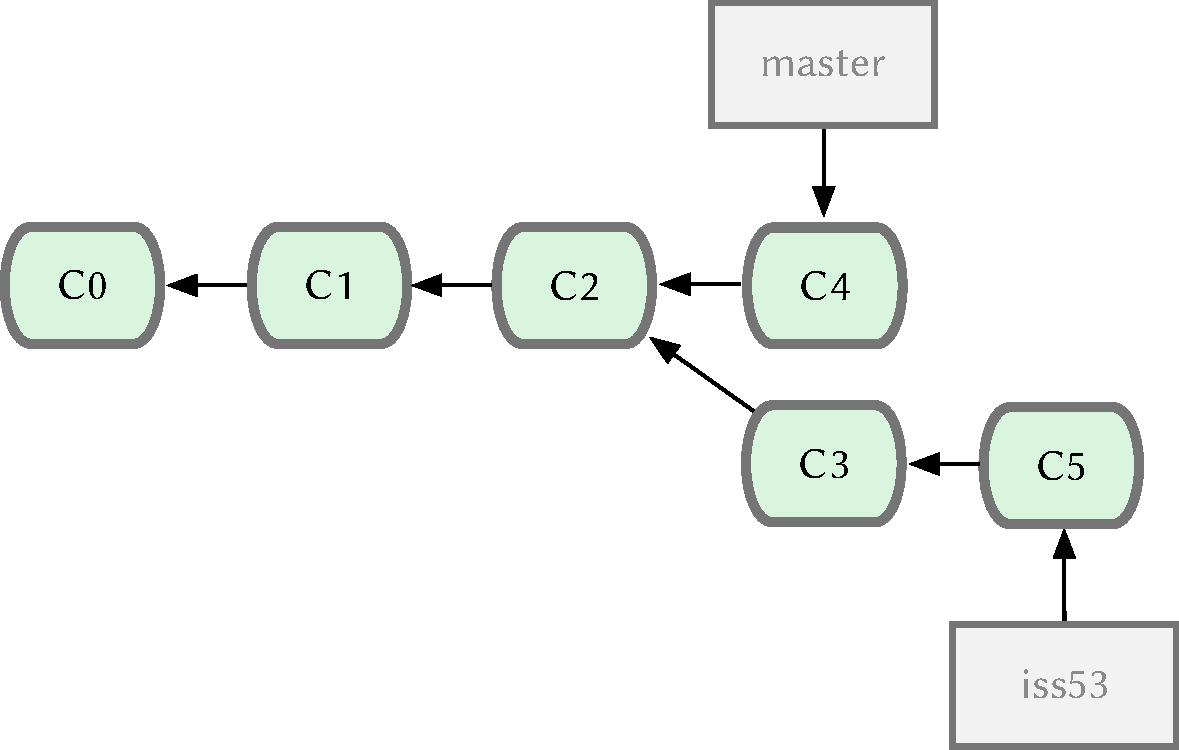
\includegraphics[scale=0.4]{images/fig0315.pdf}}
    \only<+>{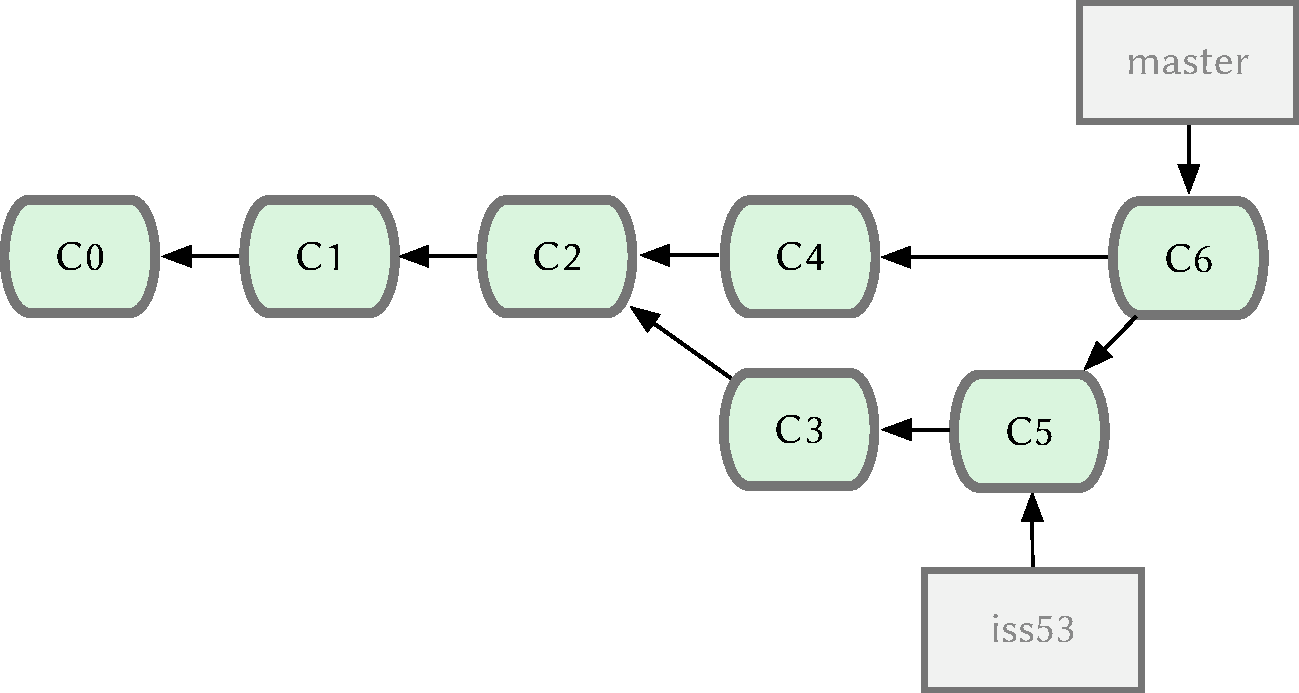
\includegraphics[scale=0.4]{images/fig0317.pdf}}
  \end{center}
  \begin{itemize}
  \item Merge iss53 into master: find best common ancestor of both branches then create a \emph{merge commit} to hold the result
  \item Conflicts happen when the same part of the same file is changed differently in both branches
  \end{itemize}
\end{frame}

\begin{frame}{Rebasing: a cleaner way to integrate changes}
  \only<+>{
    \begin{columns}[c]
      \begin{column}{5cm}
        \begin{center}
          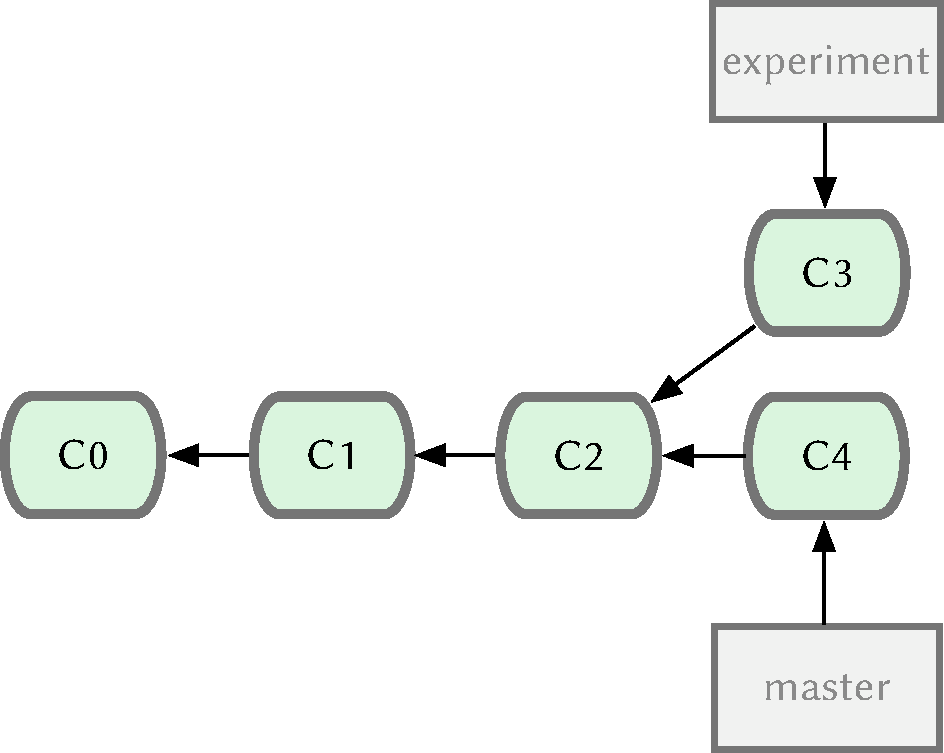
\includegraphics[scale=0.26]{images/fig0327.pdf}\\1) Initial situation: two divergent branches
        \end{center}
      \end{column}
      \begin{column}{6cm}
        \begin{center}
          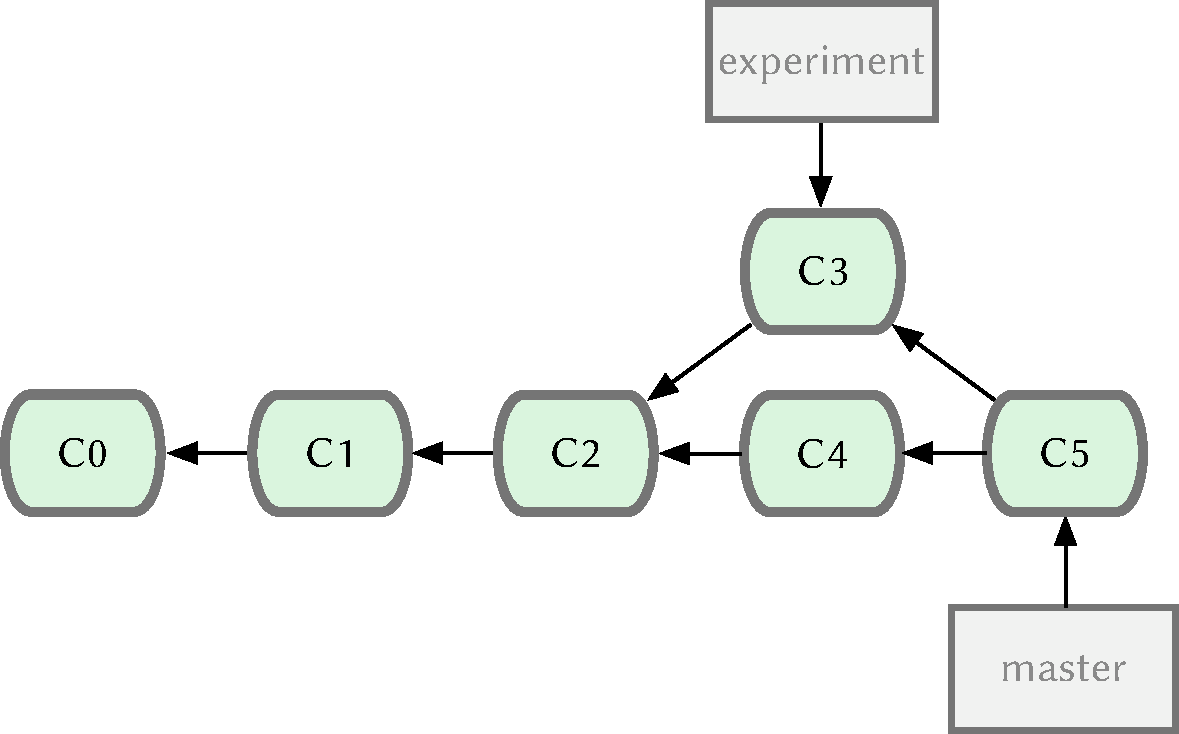
\includegraphics[scale=0.26]{images/fig0328.pdf}\\2a) \emph{Merge} experiment into master
          \vskip 0.8em
          \hrule
          \vskip 0.8em
          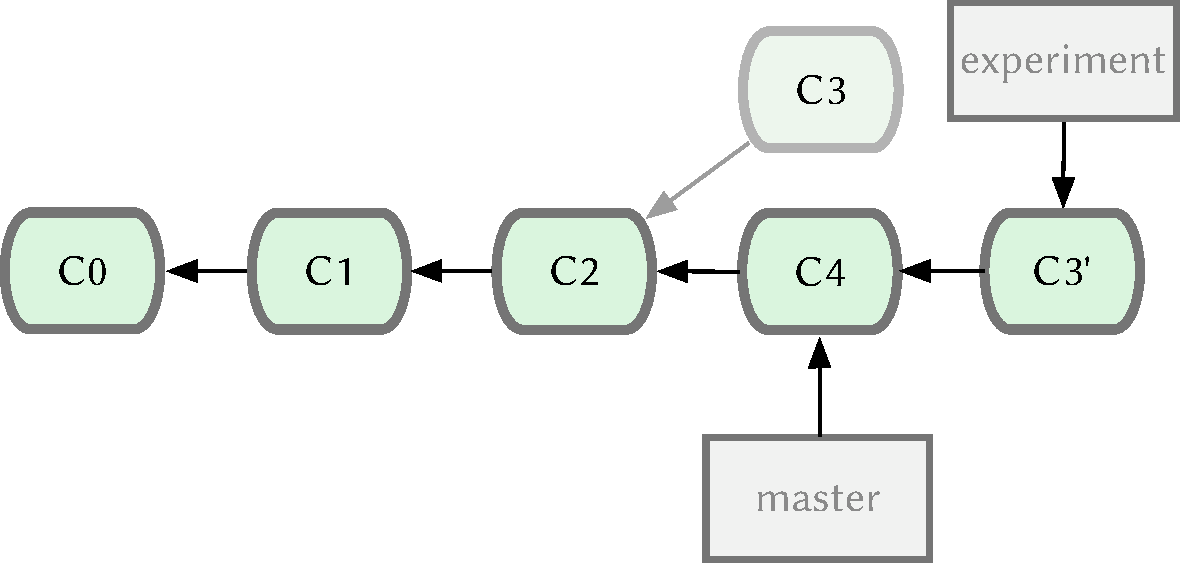
\includegraphics[scale=0.26]{images/fig0329.pdf}\\2b) \emph{Rebase} experiment onto master
        \end{center}
      \end{column}
    \end{columns}
  }
  \only<+>{
    \begin{center}
      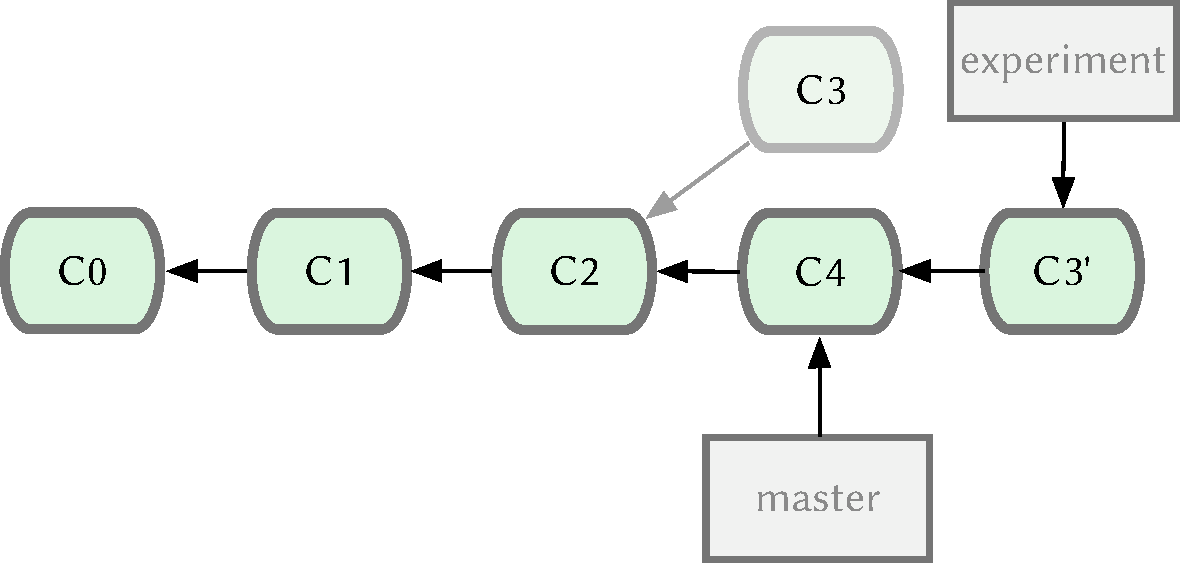
\includegraphics[scale=0.3]{images/fig0329.pdf}
    \end{center}
    \begin{itemize}
    \item Take changes from one branch (C3) and replay them on top of another branch (C4), no additional merge commit created
    \item Branches can then be merged with a fast-forward
    \item History looks linear, easier to follow
    \item Can be used to make sure changes apply cleanly on a remote branch (rebase master onto origin/master)
    \item \alert{Do not rebase commits you have already pushed!}
    \end{itemize}
  }
\end{frame}

\section{Git commands}

\subsection{Basics}

\begin{frame}{Repository creation}
  \begin{block}{Initializing a repository in an existing directory}
    \texttt{git init}
    \begin{itemize}
    \item Creates the .git directory
    \item But doesn't track any files yet
    \end{itemize}
  \end{block}
  \begin{block}{Cloning an existing repository}
    \texttt{git clone <URL>}
    \begin{itemize}
    \item Copies all data from the source repository
    \item Checks out the latest version
    \item Supports several protocols: HTTP, SSH, Git
    \end{itemize}
  \end{block}
\end{frame}

\begin{frame}{Recording changes}
  \begin{block}{Staging}
    \texttt{git add <file>}
    \begin{itemize}
    \item Adds the current state of the file to the staging area
    \item If you modify the file after \texttt{git add}, the \alert{new changes are not staged}.
    \note{Advanced: Can also add only a part of a change to the staging area, interactive option.}
    \end{itemize}
  \end{block}
  \begin{block}{Committing}
    \texttt{git commit}
    \begin{itemize}
    \item Writes staged changes to the repository
    \end{itemize}
    \texttt{git commit -a}
    \begin{itemize}
    \item Shortcut to skip the staging area
    \item Automatically stages every tracked file before doing the commit
    \end{itemize}
  \end{block}
\end{frame}

\begin{frame}{Knowing where you are}
  \begin{block}{Checking the status of your working directory}
    \texttt{git status}
    \begin{itemize}
    \item Branch currently checked out, with remote tracking information
    \item Lists files by state (staged, not staged, untracked)
    \item The most useful command to know the current state of your working directory
    \item Gives hints on what to do next or how to undo changes
    \end{itemize}
  \end{block}
\end{frame}

\begin{frame}{Looking at changes}
  \begin{block}{Viewing changes inside tracked files}
    \texttt{git diff}
    \begin{itemize}
    \item Shows what is changed but not yet staged
    \item Compares working directory with staging area
    \end{itemize}
    \texttt{git diff --staged}
    \begin{itemize}
    \item Shows what would go into the next commit
    \item Compares last commit with staging area
    \end{itemize}
  \end{block}
\end{frame}

\begin{frame}{(Re)Moving files around}
  \begin{block}{Renaming files}
    \texttt{git mv <old name> <new name>}
    \begin{itemize}
    \item Renames the file and stages the change
    \end{itemize}
  \end{block}
  \begin{block}{Removing files}
    \texttt{git rm <file>}
    \begin{itemize}
    \item Deletes the file and stages its removal
    \end{itemize}
  \end{block}
\end{frame}

\begin{frame}{Ooops! Undoing}
  \begin{block}{Changing your last commit}
    \texttt{git commit --amend}
    \begin{itemize}
    \item Adds staged files to the \alert{last} commit
    \item Edit \alert{last} commit's message
    \item Do not use this on a commit that you have already pushed!
    \end{itemize}
  \end{block}
  \begin{block}{Reverting a modified file}
    \texttt{git checkout -- <file>}
    \begin{itemize}
    \item Discards all uncommitted changes in file
    \item Reverts the file as it was in the last commit
    \end{itemize}
  \end{block}
  \begin{block}{Unstaging a staged file}
    \texttt{git reset HEAD <file>}
    \begin{itemize}
    \item Undo \texttt{git add}
    \end{itemize}
  \end{block}
\end{frame}

\begin{frame}{History}
  \begin{block}{Viewing the commit history}
    \texttt{git log}
    \begin{itemize}
    \item Lists commits from most recent to oldest
    \item Shows commit hash, author, date and message by default
    \item Has many options to customise output:
      \begin{itemize}
      \item[patch] Show what changed inside files (like \texttt{diff -u})
      \item[oneline] Prints one line per commit (only hash and summary)
      \item[decorate] Adds branch and tag names on the commit they point to
      \item[graph] Builds a visual representation of branches
      \item[stat] Adds statistics about changed files to every commit
      \end{itemize}
      Quick summary example:\\\texttt{git log --oneline --decorate --graph}
    \end{itemize}
  \end{block}
\end{frame}

\begin{frame}{Labeling commits with tags}
  \begin{block}{Listing tags}
    \texttt{git tag}
    \begin{itemize}
    \item Lists all tags in alphabetical order
    \end{itemize}
    \texttt{git show <tag>}
    \begin{itemize}
    \item Prints tag data and commit information
    \end{itemize}
  \end{block}
  \begin{block}{Creating tags}
    \texttt{git tag <name>}
    \begin{itemize}
    \item Creates a \emph{lightweight} tag: like a fixed branch pointer
    \end{itemize}
    \texttt{git tag --annotated <name>}
    \begin{itemize}
    \item Creates an \emph{annotated} tag: like a commit, has a message and can be signed
    \end{itemize}
    \texttt{git tag <name> <commit>}
    \begin{itemize}
    \item Tags can be created later on any commit
    \end{itemize}
  \end{block}
\end{frame}

\subsection{Branching and merging}

\begin{frame}{Navigating branches}
  \only<+>{
    \begin{block}{List of all branches}
      \texttt{git branch [--list] --all}
      \begin{itemize}
      \item Lists both remote-tracking and local branches
      \item Current branch is indicated with an asterisk
      \end{itemize}
    \end{block}
    \begin{block}{Creating a new branch}
      \texttt{git branch <name>}
      \begin{itemize}
      \item Creates a branch pointing to the current branch
      \item Only creates a pointer: no files are modified
      \end{itemize}
    \end{block}
    \begin{block}{Deleting a branch}
      \texttt{git branch --delete <name>}
      \begin{itemize}
      \item Branch to delete must be merged in its upstream branch
      \end{itemize}
    \end{block}
  }
  \only<+>{
    \begin{block}{Switching to another branch}
      \texttt{git checkout <branch name>}
      \begin{itemize}
      \item Changes files in working directory
      \item Working directory must be clean before switching (no uncommitted changes)
      \end{itemize}
      \texttt{git checkout -b <new branch name>}
      \begin{itemize}
      \item Shortcut to directly switch to a new branch
      \end{itemize}
    \end{block}
  }
\end{frame}

\begin{frame}{Merging}
    \begin{block}{Merging two branches}
      \texttt{git checkout <branch to merge into>}\\
      \texttt{git merge <branch to merge>}
      \begin{itemize}
      \item Merges changes from given branch into \emph{current} branch
      \item Conflicts can happen
      \end{itemize}
    \end{block}
    \begin{block}{Rebasing}
      \texttt{git rebase <upstream branch>}
      \begin{itemize}
      \item Replays commits on upstream branch
      \item Conflicts can also happen
      \end{itemize}
      \texttt{git rebase --interactive <upstream branch>}
      \begin{itemize}
      \item Review commits to be replayed (reorder, reword, squash, \ldots)
      \end{itemize}
    \end{block}
\end{frame}

\subsection{Interacting with others}

\begin{frame}{Interacting with others}
  \only<+>{
    \begin{block}{Managing links to remote repositories}
      \texttt{git remote [--verbose]}
      \begin{itemize}
      \item \emph{Remote repositories}: other versions of your project hosted elsewhere
      \item Lists, adds or removes links to remote repositories
      \item \emph{origin}: the repository you cloned from
      \end{itemize}
      \texttt{git remote show <name>}
      \begin{itemize}
      \item Displays detailed information about one remote
        \begin{itemize}
        \item Fetch and pull URLs
        \item Remote branches and whether they have a corresponding local branch (\emph{tracked})
        \item Local $\leftrightarrow$ remote branch mappings for push/pull
        \end{itemize}
      \end{itemize}
    \end{block}
  }
  \only<+>{
    \begin{block}{Retrieving new commits}
      \texttt{git fetch [remote name]}
      \begin{itemize}
      \item Downloads new changes from the remote
      \item Changes go into your repository (\texttt{.git})
      \item Your working directory \alert{is not modified}
      \item \texttt{git status} now informs about branch divergence
      \end{itemize}
    \end{block}
    \begin{block}{Updating your working directory}
      \texttt{git pull [--rebase]}
      \begin{itemize}
      \item Shortcut: downloads and merges changes = fetch + merge
      \item Your working directory \alert{is modified}
      \item With rebase = fetch + rebase
      \item Conflicts can happen, check with fetch first
      \end{itemize}
    \end{block}
  }
  \only<+>{
    \begin{block}{Sharing your commits}
      \texttt{git push [remote name] [branch name]}
      \begin{itemize}
      \item Sends your changes to the remote repository
      \item \alert{Do not use without arguments}, it pushes more than you think!\\\ldots unless you use Git version 2.0 or later
        \begin{itemize}
        \item[$v < 2.0$] Push all matching branches (same local and remote names)
        \item[$v \geqslant 2.0$] Push current branch only if remote matches
        \end{itemize}
      \end{itemize}
    \end{block}
    \begin{block}{Push rejected!}
      \begin{itemize}
      \item Commits rejected if not a fast-forward merge
      \item Must fetch new commits and merge/rebase before pushing again
      \end{itemize}
    \end{block}
  }
\end{frame}

\subsection{Documentation}

\begin{frame}{Where is the manual?}
  \begin{columns}[t]
    \begin{column}{7cm}
      \begin{block}{Built-in help}
        \texttt{git help <command>}
      \end{block}
      \begin{block}{\emph{Pro Git} book}
        \begin{itemize}
        \item \url{http://git-scm.com/book}
        \item Chapters 1--3, 5
        \end{itemize}
      \end{block}
      \begin{block}{More}
        \begin{itemize}
        \item \url{http://git-scm.com/doc}
        \item Reference
        \item Videos
        \end{itemize}
      \end{block}
    \end{column}
    \begin{column}{3cm}
      \begin{center}
        
\includegraphics[width=3cm]{images/progit2.png}
      \end{center}
    \end{column}
  \end{columns}
\end{frame}

\begin{frame}{Tips and tricks}
  \begin{block}{Stage only some parts of a file}
    \texttt{git add --patch <file>}
  \end{block}
  \begin{block}{Delete a branch on the server}
    \texttt{git push origin --delete <branch>}
  \end{block}
  \begin{block}{Commit for someone else}
    \texttt{git commit --author=<author>}
  \end{block}
\end{frame}

\section{Good practices}

%TODO: good practices, tricks
% - rebase for clean history
% - branch TTL
% - push often

\begin{frame}{Pick your work flow}
  \begin{columns}[c]
    \begin{column}{5cm}
      \begin{center}
        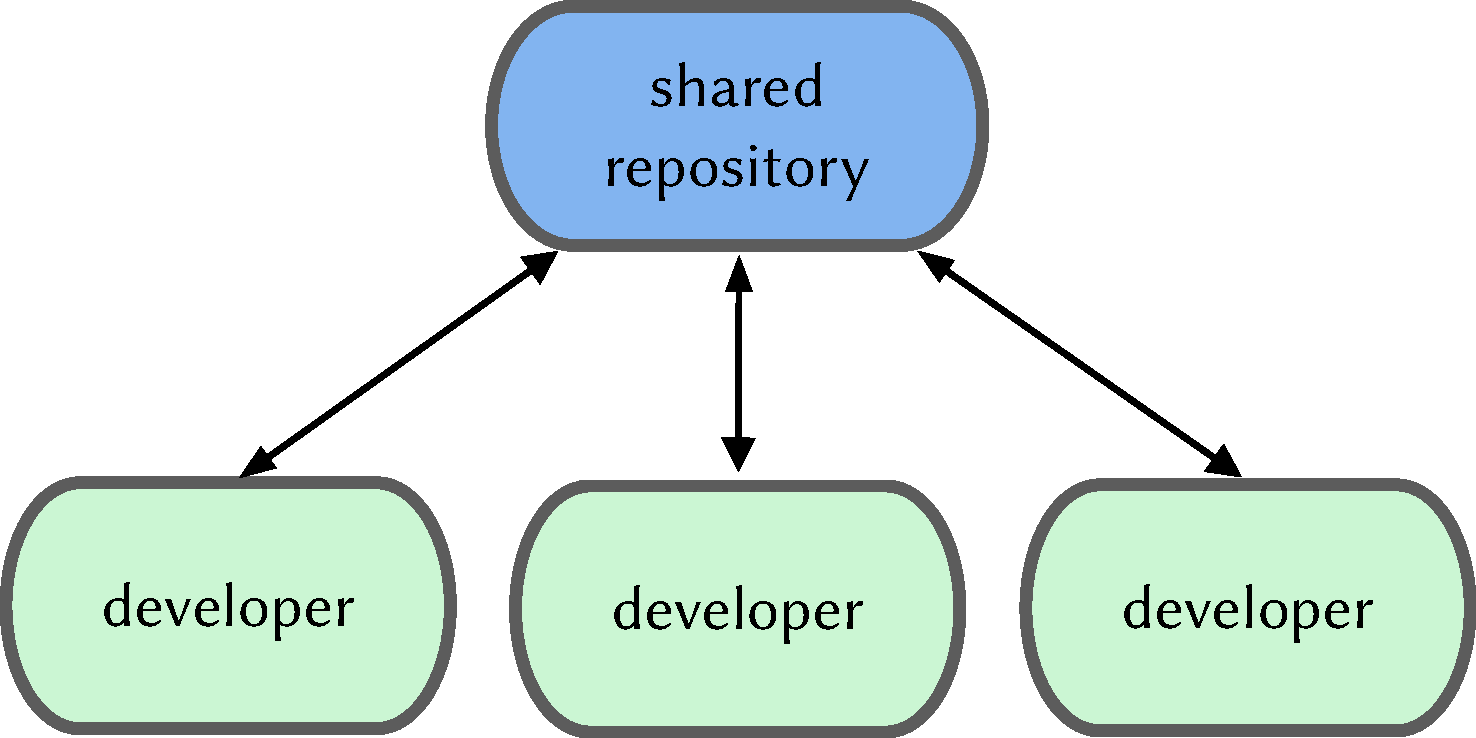
\includegraphics[width=5cm]{images/fig0501.pdf}\\Centralised
      \end{center}
    \end{column}
    \begin{column}{6cm}
      \begin{center}
        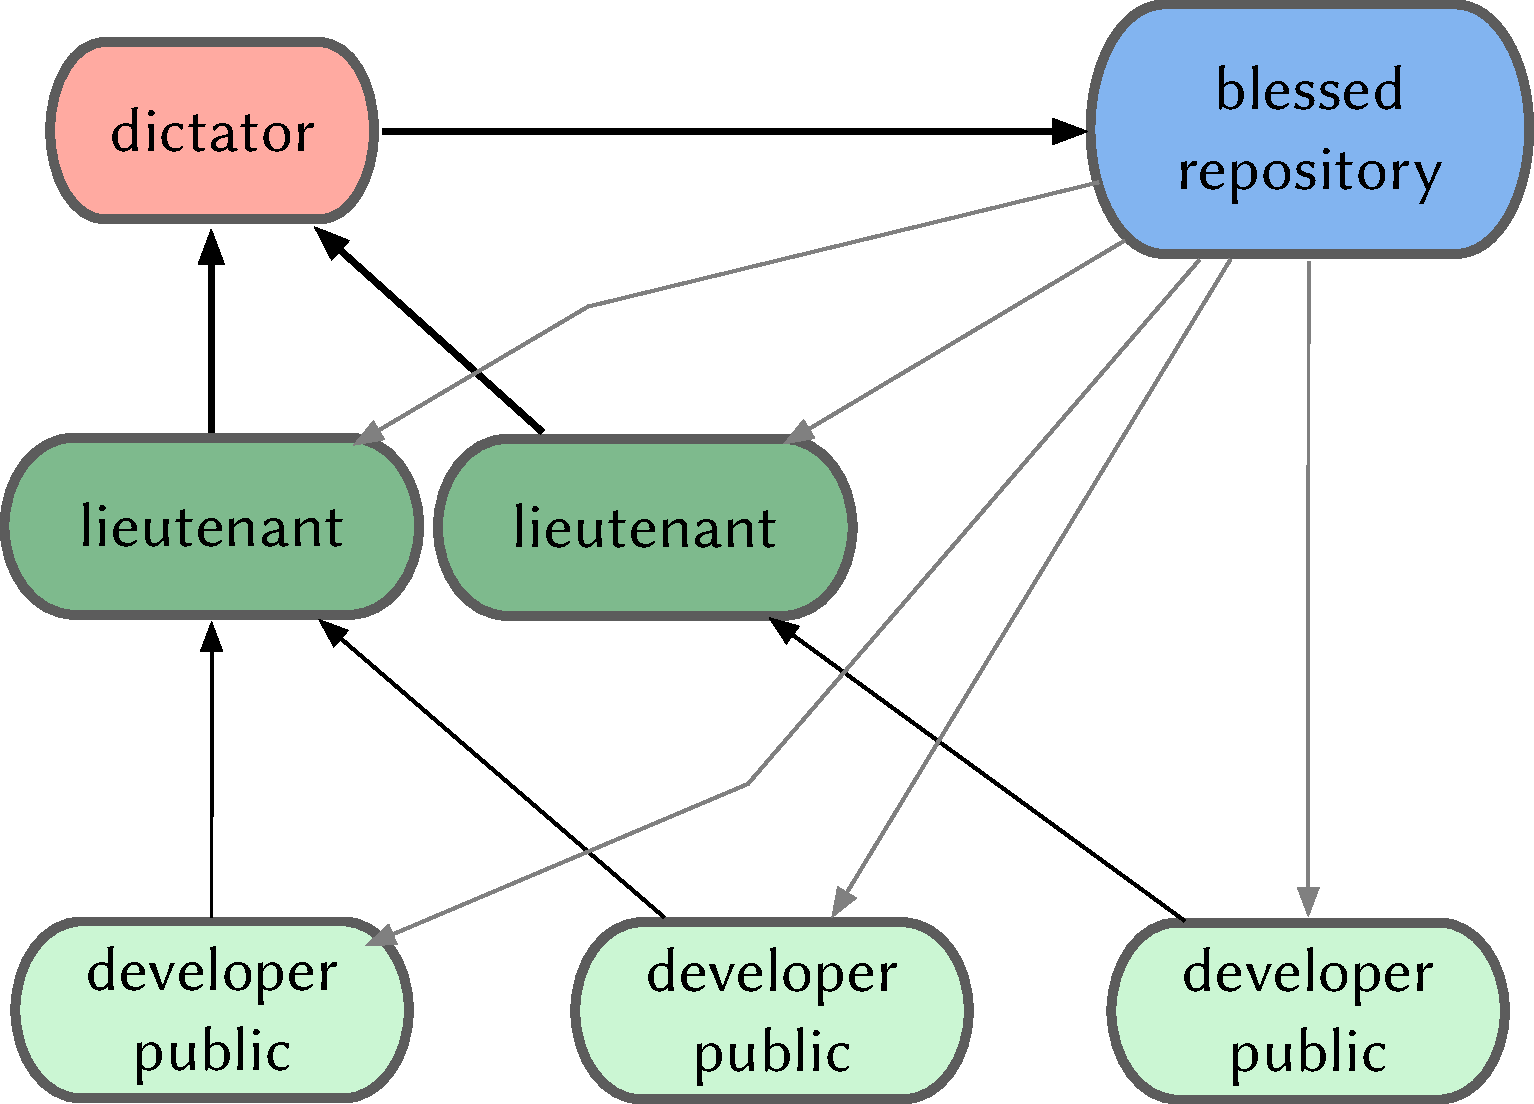
\includegraphics[width=5cm]{images/fig0503.pdf}\\Dictator and lieutenants
      \end{center}
    \end{column}
  \end{columns}
  \begin{columns}[c]
    \begin{column}{8cm}
      \begin{center}
        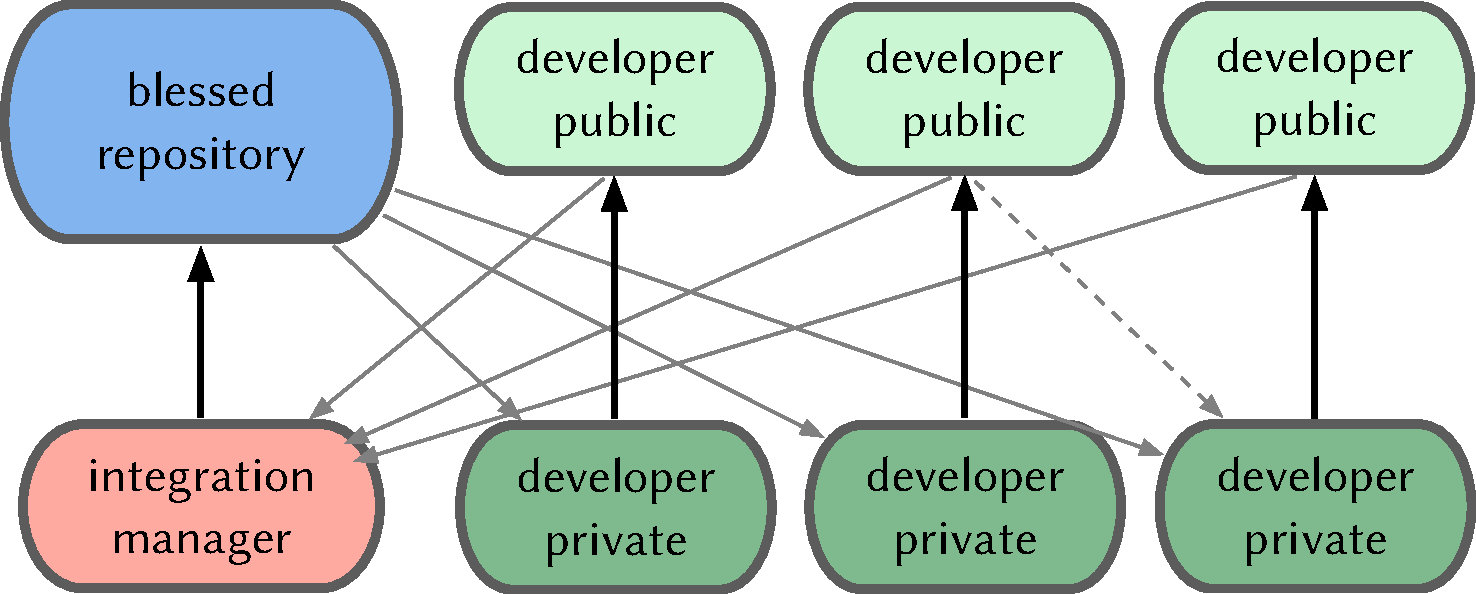
\includegraphics[width=7cm]{images/fig0502.pdf}\\Integration manager
      \end{center}
    \end{column}
  \end{columns}
\end{frame}

\begin{frame}{Commit guidelines}
  \only<+>{
    \begin{block}{Whitespace errors}
      \begin{itemize}
      \item No trailing whitespace\\Tends to annoy developers\\Run \texttt{git diff --check} before committing
      \item Verify indentation, spaces vs. tabs
      \end{itemize}
    \end{block}
    \begin{block}{Size: what goes in \emph{one} commit?}
      \begin{itemize}
      \item Commits should be ``small''
      \item Logically separate set of changes
      \item Easier to review or revert
        % TODO see rewriting history
      \end{itemize}
    \end{block}
  }
  \only<+>{
    \begin{block}{The commit message}
      \begin{enumerate}
      \item Summary, like email subject\\About 50 characters maximum
      \item \emph{blank line}
      \item Detailed explanation: motivation, implementation changes, etc.\\Lists and paragraphs are fine\\Wrapped to 72 characters per line
      \item Tracking number
      \end{enumerate}
      \begin{itemize}
      \item Imperative present tense ``Add tests for \ldots''
      \item Your contribution to project history, think of your future self!
      \item Tools rely on this formatting
      \end{itemize}
    \end{block}
  }
\end{frame}

\begin{frame}{Daily work flow}
  \begin{block}{Update your repository}
    \begin{itemize}
    \item No uncommitted changes nor unpushed commits\\$\rightarrow$ \texttt{git pull}
    \item Unpushed commits\\$\rightarrow$ \texttt{git pull --rebase}
    \item Uncommitted changes or cautious\\$\rightarrow$ \texttt{git fetch; git status}
    \end{itemize}
  \end{block}
  \begin{block}{Push often}
    \begin{enumerate}
    \item Rearrange and clean up your commits\\$\rightarrow$ \texttt{git rebase --interactive}
    \item Push shared branches to the reference repository\\$\rightarrow$ \texttt{git push origin master}
    \end{enumerate}
  \end{block}
\end{frame}

\begin{frame}{Rewriting and improving history}
  \begin{block}{The interactive rebase}
    \texttt{git rebase --interactive}
    \begin{itemize}
    \item Reorder commits
    \item Edit files or message
    \item Squash several commits into one
    \item Split a commit into several commits
    \item Drop commits
    \end{itemize}
    Reminder: this works well only on commits that are \alert{not yet pushed} elsewhere
  \end{block}
\end{frame}

\section{Hands-on}
% Use the testing repository to play with branches
% - create, switch, merge and delete
% - push and pull
% - trigger merge conflicts and resolve them
% - rebase and look at history

\end{document}
